% Compilar con: xelatex informe_clasificacion_sagital.tex (dos pasadas)
\documentclass[10pt,twocolumn,a4paper]{article}

\usepackage{fontspec}
\setmainfont{Latin Modern Roman}
\usepackage[top=2.2cm,bottom=2.2cm,left=1.9cm,right=1.9cm,columnsep=0.7cm]{geometry}
\usepackage{amsmath,amssymb}
\usepackage{booktabs}
\usepackage{graphicx}
\usepackage[font=small,labelfont=bf,labelsep=period]{caption}
\usepackage{microtype}
\usepackage{xcolor}
\usepackage{url}
\usepackage[colorlinks=true,linkcolor=blue!50!black,citecolor=blue!50!black,urlcolor=blue!50!black,pdfborder={0 0 0}]{hyperref}

% Sin babel-español en este sistema: se fijan los nombres a mano.
\renewcommand{\abstractname}{Resumen}
\renewcommand{\figurename}{Figura}
\renewcommand{\tablename}{Tabla}
\renewcommand{\refname}{Referencias}

\setlength{\parindent}{1.1em}
\setlength{\parskip}{0pt}
\renewcommand{\arraystretch}{1.12}

\newcommand{\auc}{\mathrm{AUC}}

\title{\textbf{Clasificación de marcha sagital en niños con parálisis cerebral frente a controles:\\ evaluación con validación cruzada agrupada por sujeto}}
\author{Equipo de Investigación EAFIT}
\date{Noviembre de 2026}

\makeatletter
\begin{document}
\twocolumn[
  \begin{@twocolumnfalse}
    \maketitle
    \begin{center}\textbf{\abstractname}\end{center}
    \begin{quote}\small
    \noindent
    Se estudia si las curvas cinemáticas sagitales de cadera, rodilla y tobillo, obtenidas por estimación de pose en video y normalizadas al ciclo de marcha, permiten distinguir a niños con parálisis cerebral (17 sujetos) de niños con marcha típica (39 sujetos). Se comparan un Random Forest sobre 36 biomarcadores por ciclo y una red convolucional 1D sobre las curvas completas. Dado el tamaño muestral, la evaluación usa validación cruzada estratificada, repetida y agrupada por sujeto, con ponderación por sujeto, y se informa el AUC a nivel paciente con intervalos de confianza por bootstrap. El Random Forest alcanza un AUC de $0.79 \pm 0.04$ (IC95\,\% orientativo ${[0.68, 0.93]}$) y la red convolucional $0.65 \pm 0.03$. Estos valores indican una señal discriminativa moderada, no un desempeño diagnóstico: el número de casos es bajo, 12 sujetos del conjunto original quedaron fuera por falta de ciclos procesados, y no se identificaron biomarcadores individuales determinantes. Se discuten las limitaciones y los pasos necesarios antes de cualquier uso clínico.
    \medskip

    \noindent\textbf{Palabras clave:} parálisis cerebral, marcha, cinemática sagital, validación cruzada agrupada, Random Forest, red convolucional 1D, AUC.
    \end{quote}
    \vspace{0.6em}
  \end{@twocolumnfalse}
]
\makeatother

\section{Introducción}

El análisis cuantitativo de la marcha permite describir las alteraciones motoras asociadas a la parálisis cerebral (PC) y es una entrada habitual en trabajos de clasificación automática, como la clasificación de formas de diplejía con redes LSTM sobre datos de captura con marcadores \cite{ferrari2019}. Una alternativa de menor costo es estimar los ángulos articulares a partir de video, pero esa señal es más ruidosa y rara vez se evalúa con el rigor que exigen los conjuntos de datos pequeños.

Este trabajo aborda una pregunta acotada: \emph{¿contienen las curvas sagitales normalizadas de cadera, rodilla y tobillo información suficiente para separar a niños con PC de niños con marcha típica?} Las contribuciones son metodológicas más que de desempeño: (i) un protocolo de evaluación a nivel de sujeto que evita la fuga de información entre ciclos de un mismo niño, (ii) la comparación de un modelo interpretable y uno de aprendizaje profundo bajo el mismo protocolo y (iii) una descripción explícita de lo que estos resultados \emph{no} permiten concluir.

\section{Datos}

Los datos provienen de grabaciones de marcha de una sola cámara sagital (\texttt{cam1}, una sesión por sujeto) procesadas mediante estimación de pose, a unos 30\,Hz. Para cada trial se dispone de ciclos de marcha segmentados y normalizados a 101 puntos (0--100\,\% del ciclo) para seis señales: flexión de cadera, rodilla y tobillo, izquierda y derecha.

Se construye una muestra por \emph{ciclo bilateral}, emparejando el ciclo $k$ del lado izquierdo con el ciclo $k$ del derecho. Estos no corresponden al mismo paso (sus inicios difieren en torno a medio ciclo), por lo que las características de asimetría comparan zancadas consecutivas y no simultáneas. Solo se conservan ciclos con ambos lados y las seis señales completas.

El archivo de asignación de grupos lista 68 sujetos (27 casos, 41 controles). De ellos, 12 (10 casos y 2 controles) carecen de ciclos normalizados bilaterales en el procesamiento previo y quedan fuera del análisis; el origen de esa omisión no se investigó aquí. La Tabla~\ref{tab:datos} resume la muestra analizada.

\begin{table}[t]
\centering\small
\caption{Muestra analizada (tras excluir 12 sujetos sin ciclos normalizados).}
\label{tab:datos}
\begin{tabular}{lrr}
\toprule
 & Control & Caso (PC) \\
\midrule
Sujetos & 39 & 17 \\
Trials & 40 & 17 \\
Ciclos bilaterales & 160 & 52 \\
Ciclos por sujeto (media) & 4.1 & 3.1 \\
\bottomrule
\end{tabular}
\end{table}

Cada sujeto aporta uno o varios ciclos, fuertemente correlacionados entre sí; el tamaño muestral efectivo es por tanto cercano a 56 y no a 212. Además, los controles aportan más ciclos por sujeto que los casos, lo que justifica la ponderación descrita en la Sección~\ref{sec:pesos}.

\section{Métodos}

\subsection{Representaciones de entrada}

\textbf{Curvas.} Cada ciclo es un tensor $X \in \mathbb{R}^{6\times 101}$, normalizado por canal con la media y la desviación estándar del conjunto de entrenamiento antes de entrar a la red convolucional.

\textbf{Biomarcadores.} Para cada una de las seis señales se calculan cinco estadísticos del ciclo (media, desviación estándar, mínimo, máximo y rango de movimiento, $\mathrm{ROM}=\max\theta-\min\theta$), lo que da 30 características. Se añaden seis de asimetría entre extremidades, para cada articulación $a\in\{\text{cadera},\text{rodilla},\text{tobillo}\}$:
\begin{gather}
A^{\mathrm{ROM}}_a = \bigl|\mathrm{ROM}_{a,\mathrm{izq}}-\mathrm{ROM}_{a,\mathrm{der}}\bigr|,\\
A^{\mathrm{media}}_a = \bigl|\bar\theta_{a,\mathrm{izq}}-\bar\theta_{a,\mathrm{der}}\bigr|.
\end{gather}
El vector final tiene 36 dimensiones.

\subsection{Modelos}

\textbf{Random Forest} \cite{breiman2001}: 150 árboles de profundidad máxima 6 sobre los 36 biomarcadores.

\textbf{GaitCNN1D}: tres bloques convolucionales 1D (32, 64 y 128 filtros; núcleos 5, 5 y 3) con normalización por lotes, ReLU y \emph{max pooling} en los dos primeros, \emph{pooling} promedio global y un clasificador de dos capas lineales (32 unidades) con \emph{dropout} de 0.3. Se entrena con AdamW (tasa de aprendizaje $10^{-3}$, decaimiento de pesos $10^{-3}$), lotes de 16 y hasta 60 épocas, con detención temprana (paciencia 10) según la pérdida de un conjunto de validación interno formado por el 20\,\% de los \emph{sujetos} del entrenamiento. El conjunto de prueba nunca interviene en el ajuste.

Ambos modelos se implementaron con scikit-learn \cite{pedregosa2011} y PyTorch \cite{paszke2019}.

\subsection{Ponderación por sujeto}
\label{sec:pesos}

Sea $s(i)$ el sujeto del ciclo $i$ y $n_s$ su número de ciclos. Cada ciclo recibe un peso $w_i = c_{y_i}/n_{s(i)}$, con constantes $c_0, c_1$ tales que cada clase suma el mismo peso total. Así ningún niño influye más por tener más ciclos y las clases quedan balanceadas a nivel sujeto, no a nivel ciclo. Los pesos se usan en el ajuste del Random Forest y en la pérdida de entropía cruzada de la red.

\subsection{Validación cruzada agrupada por sujeto}

La evaluación usa validación cruzada de 4 particiones, estratificada por clase y repetida 5 veces con repartos distintos (20 ajustes por modelo). La unidad de reparto es el \emph{sujeto}: todos los ciclos de un niño quedan en el mismo lado de la partición, lo que se verifica explícitamente. En cada repetición cada niño se evalúa exactamente una vez con un modelo que no lo vio durante el entrenamiento.

\subsection{Métricas}

La probabilidad de un sujeto $s$ es el promedio de las de sus ciclos de prueba, $\bar p_s = n_s^{-1}\sum_{i\in s} p_i$. La métrica principal es el \textbf{AUC a nivel paciente}, calculado sobre los 56 sujetos en cada repetición; se informa su media y desviación entre repeticiones (variabilidad por el reparto). Además se reporta un IC95\,\% por bootstrap percentil que remuestrea sujetos con reemplazo \cite{efron1993} sobre $\bar p_s$ promediada entre repeticiones. Este intervalo es orientativo: el promedio entre repeticiones reduce la varianza de las predicciones y lo centra por encima de la media por repetición.

De forma secundaria se reportan sensibilidad, especificidad y exactitud balanceada con umbral fijo $0.5$, \emph{sin calibrar}. Esas métricas dependen del corte y de cómo cada modelo calibra sus probabilidades, por lo que no se usan para comparar modelos.

\subsection{Importancia de características}

Para el Random Forest se calcula la importancia por permutación: en cada partición de prueba se baraja una característica entre los ciclos (10 veces) y se mide la caída del AUC por ciclo; el resultado se promedia entre las 20 particiones. A diferencia de la importancia de Gini, se mide con datos no vistos en el entrenamiento y no depende de la cardinalidad de la variable.

\section{Resultados}

\subsection{Descripción de las curvas}

La Figura~\ref{fig:curvas} muestra la media entre sujetos de cada grupo. Las bandas de $\pm1$ desviación estándar entre sujetos se solapan en gran parte del ciclo en las seis señales, lo que anticipa una separación imperfecta. A nivel de biomarcadores (Figura~\ref{fig:bio}), el ROM de cadera y rodilla izquierdas se solapa ampliamente entre grupos, mientras que la asimetría de ROM de rodilla tiende a ser mayor en los casos; no se contrastó formalmente.

\begin{figure*}[t]
\centering
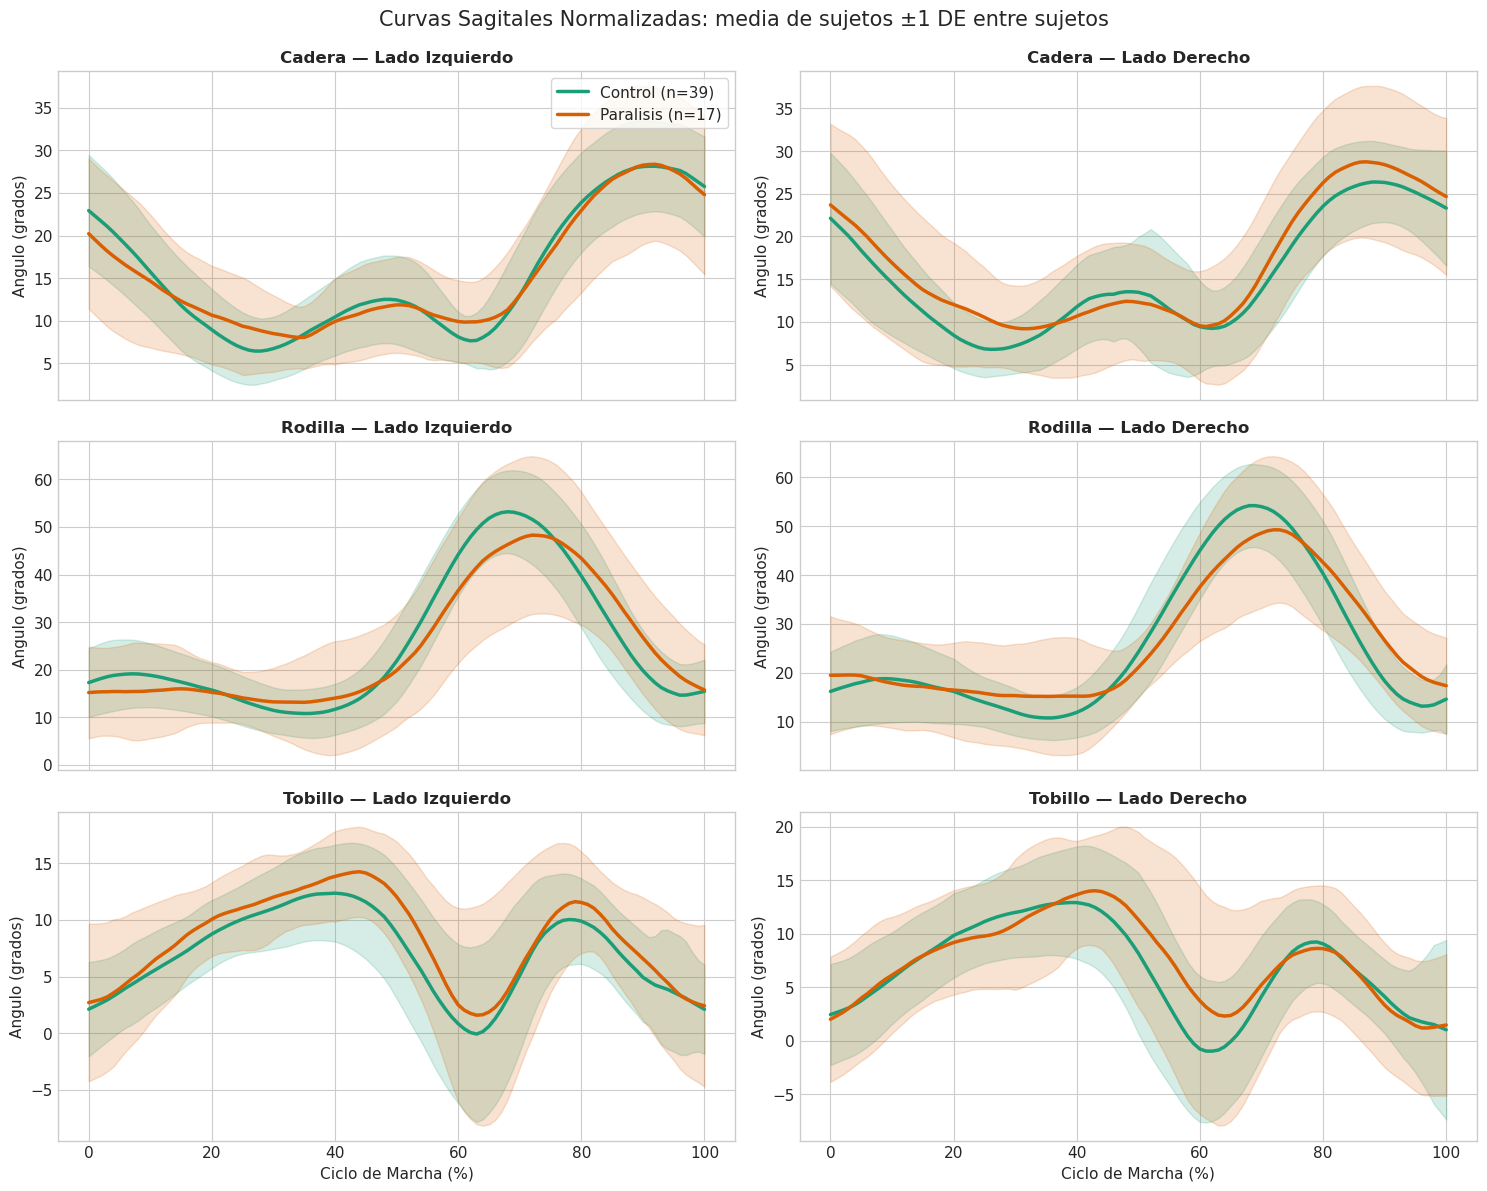
\includegraphics[width=0.78\textwidth]{figures/curvas_medias.png}
\caption{Curvas sagitales normalizadas: media entre sujetos $\pm1$ desviación estándar entre sujetos (control $n=39$, caso $n=17$).}
\label{fig:curvas}
\end{figure*}

\begin{figure*}[t]
\centering
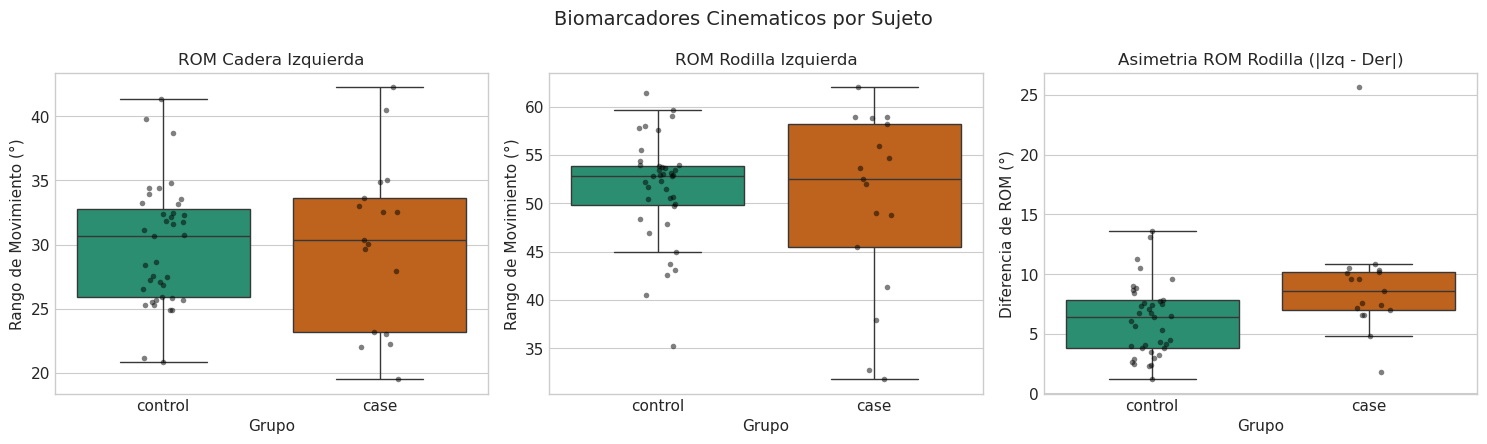
\includegraphics[width=0.85\textwidth]{figures/biomarcadores.png}
\caption{Biomarcadores promediados por sujeto (un punto por niño).}
\label{fig:bio}
\end{figure*}

\subsection{Desempeño a nivel paciente}

\begin{table}[t]
\centering\small
\caption{AUC a nivel paciente. Media $\pm$ DE entre las 5 repeticiones; IC95\,\% por bootstrap de sujetos (orientativo).}
\label{tab:auc}
\begin{tabular}{lcc}
\toprule
Modelo & AUC & IC95\,\% \\
\midrule
Random Forest & $0.790\pm0.035$ & $[0.68,\,0.93]$ \\
GaitCNN1D & $0.649\pm0.033$ & $[0.61,\,0.88]$ \\
\bottomrule
\end{tabular}
\end{table}

El Random Forest obtiene un AUC medio de 0.79 y la red convolucional de 0.65 (Tabla~\ref{tab:auc}, Figura~\ref{fig:roc}). Los intervalos se solapan, de modo que con 56 sujetos no es posible afirmar que un modelo sea superior; sí se observa que la red, más compleja, no mejora al modelo sobre biomarcadores.

\begin{figure}[t]
\centering
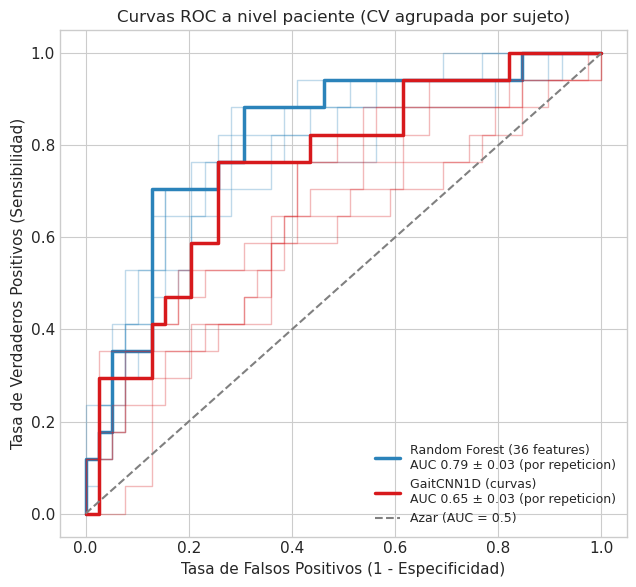
\includegraphics[width=\columnwidth]{figures/roc.png}
\caption{Curvas ROC a nivel paciente. Líneas finas: una por repetición; líneas gruesas: probabilidad promediada entre repeticiones (se ve algo mejor que el AUC por repetición de la leyenda).}
\label{fig:roc}
\end{figure}

\subsection{Métricas con umbral fijo}

\begin{table}[t]
\centering\small
\caption{Umbral fijo 0.5, sin calibrar (media entre repeticiones, nivel paciente). No es una comparación entre modelos.}
\label{tab:umbral}
\begin{tabular}{lccc}
\toprule
Modelo & Ex. bal. & Sens. & Espec. \\
\midrule
Random Forest & 0.509 & 0.024 & 0.995 \\
GaitCNN1D & 0.603 & 0.529 & 0.677 \\
\bottomrule
\end{tabular}
\end{table}

Con el corte por defecto el Random Forest casi no detecta casos (sensibilidad 0.02) pese a su AUC de 0.79, mientras que la red reparte mejor los errores (Tabla~\ref{tab:umbral}). Esto indica que el RF ordena razonablemente a los sujetos pero sus probabilidades quedan, probablemente, comprimidas hacia la clase mayoritaria: es un efecto del corte y no de la capacidad de ordenar. El umbral no se calibró, pues con 17 casos la elección sería inestable.

\subsection{Importancia de características}

La mayor caída de AUC por permutación es de unos 0.03 (\texttt{right\_hip\_std}) y en 9 de las 10 características principales la desviación entre particiones es igual o mayor que la media (Figura~\ref{fig:imp}). Ninguna característica destaca con claridad.

\begin{figure}[t]
\centering
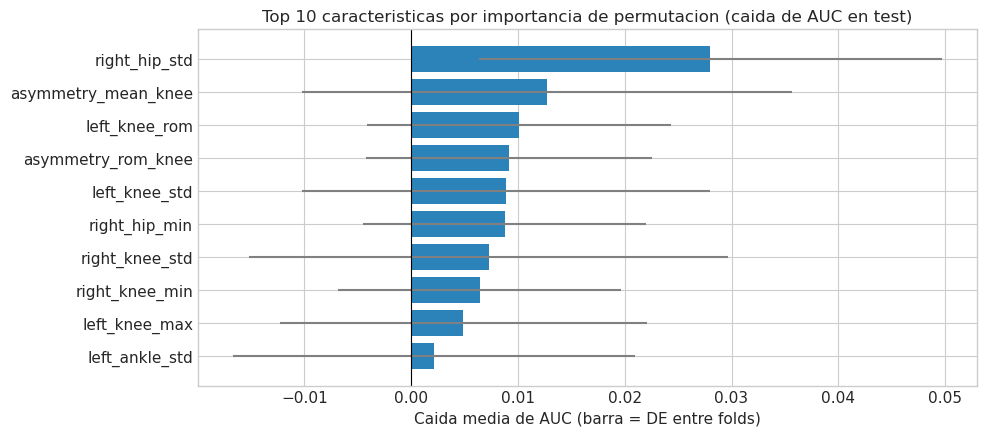
\includegraphics[width=\columnwidth]{figures/importancia.png}
\caption{Diez características con mayor importancia por permutación (caída media de AUC en prueba; barra = DE entre particiones).}
\label{fig:imp}
\end{figure}

\section{Discusión}

Los resultados apuntan a información discriminativa moderada en las curvas sagitales: el AUC del Random Forest queda claramente por encima del azar, con un intervalo que excluye 0.5, y el de la red convolucional es menor y más incierto. Un AUC de 0.79 significa que, ante un caso y un control elegidos al azar, el modelo asigna mayor probabilidad al caso en aproximadamente cuatro de cada cinco parejas; no equivale a una exactitud diagnóstica del 79\,\%.

Que la red convolucional no supere al modelo sobre biomarcadores es esperable con 56 sujetos: un modelo con decenas de miles de parámetros dispone de pocos ejemplos independientes. Tampoco puede atribuirse a los biomarcadores un papel determinante, porque la importancia por permutación es baja y ruidosa; además, al estar muy correlacionadas características de una misma señal (media, mínimo, máximo y ROM), la permutación tiende a subestimar a cada una por separado. Una versión previa de este análisis, con un único reparto de 9 sujetos de prueba (3 casos), afirmaba una alta capacidad de discriminación y atribuía el peso al ROM de rodilla y tobillo; esas afirmaciones no se sostienen con la evaluación presentada aquí.

\section{Limitaciones}

\begin{itemize}\itemsep0pt
\item \textbf{Pocos casos.} Con 17 casos y un trial por sujeto, toda estimación es inestable; faltan además 10 casos excluidos por el procesamiento previo.
\item \textbf{Sin validación externa.} Todos los registros comparten cámara y sesión; no se evaluó generalización a otros entornos o instrumentos.
\item \textbf{Señal de pose por video.} Es más ruidosa que la captura con marcadores y su error no se cuantificó.
\item \textbf{Ángulos sin signo aparente.} Cadera y rodilla no toman valores negativos en ningún grupo, lo que sugiere ángulos sin signo y limita su lectura como flexión/extensión. Debe verificarse en el procesamiento previo; por ello no se interpretan patrones clínicos concretos (equino, \emph{crouch}, rodilla rígida).
\item \textbf{Asimetría entre zancadas.} Compara ciclos izquierdo y derecho no simultáneos.
\item \textbf{IC optimista.} El bootstrap sobre probabilidades promediadas entre repeticiones subestima la incertidumbre.
\end{itemize}

\section{Conclusiones}

Con una evaluación agrupada por sujeto, ponderada y repetida, las curvas sagitales estimadas por pose muestran una señal discriminativa moderada entre niños con PC y controles (AUC de 0.79 con Random Forest y de 0.65 con una red convolucional 1D). Los datos no sustentan afirmar un desempeño diagnóstico, preferir el aprendizaje profundo ni identificar biomarcadores individuales. Los pasos siguientes son recuperar los casos excluidos, verificar la convención de signo de los ángulos y disponer de una cohorte independiente para validación externa.

\begin{thebibliography}{9}\small
\bibitem{ferrari2019} A.~Ferrari \emph{et al.}, ``Gait-based diplegia classification using LSTM networks,'' \emph{Journal of Healthcare Engineering}, 2019.
\bibitem{breiman2001} L.~Breiman, ``Random forests,'' \emph{Machine Learning}, vol.~45, no.~1, pp.~5--32, 2001.
\bibitem{pedregosa2011} F.~Pedregosa \emph{et al.}, ``Scikit-learn: Machine learning in Python,'' \emph{Journal of Machine Learning Research}, vol.~12, pp.~2825--2830, 2011.
\bibitem{paszke2019} A.~Paszke \emph{et al.}, ``PyTorch: An imperative style, high-performance deep learning library,'' in \emph{Advances in Neural Information Processing Systems}, vol.~32, 2019.
\bibitem{efron1993} B.~Efron and R.~J.~Tibshirani, \emph{An Introduction to the Bootstrap}. Chapman \& Hall, 1993.
\end{thebibliography}

\end{document}
